\documentclass[11pt]{article}

\usepackage[margin=1in]{geometry}
\usepackage[T1]{fontenc}
\usepackage{lmodern}
\usepackage{microtype}
\usepackage{amsmath,amssymb,amsthm,mathtools}
\usepackage[dvipsnames]{xcolor}
\usepackage[most]{tcolorbox}
\usepackage{tikz}
\usepackage{enumitem}
\usepackage{tocloft}
\usepackage[hidelinks]{hyperref}

\definecolor{courseblue}{HTML}{1F4E79}
\definecolor{lightblue}{HTML}{EAF2F8}
\definecolor{lightgreen}{HTML}{EAF7EA}
\definecolor{lightpink}{HTML}{FCE8EF}
\definecolor{darkgray}{HTML}{333333}

\setlength{\parindent}{0pt}
\setlength{\parskip}{0.65em}
\setlist[itemize]{topsep=0.25em,itemsep=0.15em}
\renewcommand{\cftsecleader}{\cftdotfill{\cftdotsep}}
\renewcommand{\cftsubsecleader}{\cftdotfill{\cftdotsep}}

\theoremstyle{plain}
\newtheorem{theorem}{Theorem}[section]
\newtheorem{proposition}[theorem]{Proposition}
\newtheorem{lemma}[theorem]{Lemma}
\theoremstyle{definition}
\newtheorem{definition}[theorem]{Definition}
\newtheorem{example}[theorem]{Example}
\newtheorem{exercise}[theorem]{Exercise}
\theoremstyle{remark}
\newtheorem*{remark}{Remark}

\tcolorboxenvironment{definition}{
  enhanced,
  colback=lightgreen,
  colframe=ForestGreen,
  boxrule=0.7pt,
  arc=2pt,
  left=6pt,
  right=6pt,
  top=5pt,
  bottom=5pt
}

\tcolorboxenvironment{exercise}{
  enhanced,
  colback=lightpink,
  colframe=WildStrawberry,
  boxrule=0.7pt,
  arc=2pt,
  left=6pt,
  right=6pt,
  top=5pt,
  bottom=5pt
}

\numberwithin{equation}{section}

\newcommand{\be}{\begin{eqnarray}}
\newcommand{\ee}{\end{eqnarray}}
\newcommand{\C}{\mathbb{C}}
\newcommand{\R}{\mathbb{R}}

\newcommand{\zz}{\mathbf z}
\newcommand{\ww}{\mathbf w}
\newcommand{\hh}{\mathbf h}
\DeclareMathOperator{\Real}{Re}
\DeclareMathOperator{\Imag}{Im}
\tcbset{breakable}
\begin{document}

\begin{center}
  \colorbox{lightblue}{%
    \begin{minipage}{0.94\textwidth}
      \vspace{0.55em}
      \begin{tabular*}{\textwidth}{@{\extracolsep{\fill}}lr}
        {\color{courseblue}\bfseries\LARGE Lecture 5} &
        {\color{courseblue}\bfseries\LARGE MATH 411}\\[0.35em]
        \textbf{Fall 2026} & \textbf{Date: Sep 14, 2026}\\
        & \textbf{Instructor: Manish Patnaik}
      \end{tabular*}
      \vspace{0.45em}
    \end{minipage}}
\end{center}

\setcounter{tocdepth}{1}
\tableofcontents
\vspace{0.45em}

% Handwritten page 1.
\section{Completing the proof of the Cauchy--Riemann criterion}
Last time we almost finished the proof of the following equivalence.
Throughout, $U\subseteq\C$ is open, we identify $\C$ with $\R^2$ via
$z=x+iy\leftrightarrow\zz=\begin{pmatrix}x\\y\end{pmatrix}$, and we write
\be
 f:U\to\C,\qquad f(z)=u(x,y)+iv(x,y),\qquad
 F:U\to\R^2,\qquad F=\begin{pmatrix}u(x,y)\\v(x,y)\end{pmatrix}.
\ee

\begin{theorem}[Cauchy--Riemann criterion]
\label{thm:CR}
\be
 \left\{
 \begin{array}{c}
 F\text{ is totally differentiable at }\zz\in U\\[0.3em]
 \text{and }J_F=\begin{pmatrix}u_x&u_y\\v_x&v_y\end{pmatrix}
 \text{ satisfies \emph{CR}}\\[0.3em]
 \text{(i.e. }u_x=v_y,\ u_y=-v_x\text{)}
 \end{array}
 \right\}
 \quad\Longleftrightarrow\quad
 \left\{
 \begin{array}{c}
 f(z)=u(x,y)+iv(x,y)\\[0.3em]
 \text{is }\C\text{-differentiable}\\[0.3em]
 \text{at }z\in U\subseteq\C
 \end{array}
 \right\}
\ee
\end{theorem}

The implication $(\Longleftarrow)$ was proved last time: complex
differentiability of $f$ at $z$ was shown to force total differentiability
of $F$ at $\zz$ together with the Cauchy--Riemann equations.

Let us now prove $(\Longrightarrow)$. What we must show is that there exist
a complex number $\xi=a+ib\in\C$ and a function $\sigma(w)$, defined near
$w=0$, such that
\begin{enumerate}
\item $f(z+w)-f(z)=\xi w+\sigma(w)w$;
\item $\displaystyle\lim_{w\to0}\sigma(w)=0$.
\end{enumerate}

How do we produce such a $\xi\in\C$? All we know is that
$F=\begin{pmatrix}u\\v\end{pmatrix}$ is totally differentiable at $\zz$ and
that its Jacobian satisfies the Cauchy--Riemann equations.

% Handwritten page 2.
\subsection{Producing $\xi$}
Since $F$ satisfies CR at $\zz$, the derivative matrix has the special shape
\be
 D_{\zz}=\begin{pmatrix}u_x&u_y\\v_x&v_y\end{pmatrix}
 =\begin{pmatrix}a&-b\\b&a\end{pmatrix},
 \qquad a=u_x=v_y,\quad b=v_x=-u_y,
\ee
for some $a,b\in\R$. This is precisely the matrix of multiplication by the
complex number
\be
 \boxed{\xi=a+ib\in\C.}
\ee
Indeed, if $w=h+ik$ corresponds to $\ww=\begin{pmatrix}h\\k\end{pmatrix}$, then
\be
 \xi w=(a+ib)(h+ik)=(ah-bk)+i(ak+bh),
 \qquad
 D_{\zz}\ww=\begin{pmatrix}ah-bk\\ak+bh\end{pmatrix},
\ee
so that $D_{\zz}\ww$ is exactly the pair of real and imaginary parts of
$\xi w$. Consequently the real expression
\be
 F(\zz+\ww)-F(\zz)-D_{\zz}\ww
 =\begin{pmatrix}\varphi_1(h,k)\\\varphi_2(h,k)\end{pmatrix}
\ee
matches, componentwise, the complex expression
\be
 f(z+w)-f(z)-\xi w=\varphi_1(h,k)+i\,\varphi_2(h,k).
\ee
From the definition of total differentiability of $F$ at $\zz$ we know that
\be
 \lim_{\ww\to0}\frac{\varphi_1(h,k)}{\|\ww\|}
 =\lim_{\ww\to0}\frac{\varphi_2(h,k)}{\|\ww\|}=0.
\ee

\subsection{Producing $\sigma$}
Define $\sigma(w)$ using the expression above: for $w\ne0$ set
\be
 \sigma(w)\cdot w=\varphi_1(h,k)+i\,\varphi_2(h,k),
 \qquad\text{i.e.}\qquad
 \sigma(w)=\frac{\varphi_1(h,k)+i\,\varphi_2(h,k)}{w},
\ee
and set $\sigma(0)=0$. With this definition, property (1) holds by
construction.

\begin{exercise}
Check that $\displaystyle\lim_{w\to0}\sigma(w)=0$, using the two limits
recorded above.
\end{exercise}

\begin{remark}
Here is the check. Since $|w|=\sqrt{h^2+k^2}=\|\ww\|$, for $w\ne0$,
\be
 |\sigma(w)|
 =\frac{|\varphi_1(h,k)+i\varphi_2(h,k)|}{|w|}
 =\frac{\sqrt{\varphi_1(h,k)^2+\varphi_2(h,k)^2}}{\|\ww\|}
 \le\frac{|\varphi_1(h,k)|}{\|\ww\|}+\frac{|\varphi_2(h,k)|}{\|\ww\|}
 \longrightarrow0.
\ee
Hence $\sigma(w)\to0$ as $w\to0$, which is (2). Therefore $f$ is complex
differentiable at $z$, with $f'(z)=\xi=u_x+iv_x$. \qedhere
\end{remark}

\section{A simple application: locally constant functions}
\begin{definition}
We say that $f:U\to\C$ is \emph{locally constant} if for each $z\in U$
there is a neighbourhood $D(z,\epsilon)\subseteq U$ such that
\be
 f\big|_{D(z,\epsilon)}=\text{constant}.
\ee
\end{definition}

%\begin{center}
%\begin{tikzpicture}[scale=0.9]
% % a disconnected picture: an interval in R, and two blobs
% \draw[thick] (-5.4,0)--(-1.6,0);
% \node[right] at (-1.5,0) {$\R$};
% \draw[WildStrawberry,thick] (-5.0,0.0) ellipse (0.55 and 0.22);
% \fill[WildStrawberry] (-5.0,0) circle (1.2pt);
% \draw[blue,thick] (-3.2,0.0) ellipse (0.55 and 0.22);
% \fill[blue] (-3.2,0) circle (1.2pt);
% % blob 1
% \begin{scope}[shift={(0,0)}]
%  \draw[thick] plot[smooth cycle] coordinates
%   {(-0.6,-0.7) (-0.5,0.5) (0.1,0.8) (0.5,0.1) (0.3,-0.8)};
%  \draw[WildStrawberry] (-0.35,-0.55)--(-0.1,0.6);
%  \draw[WildStrawberry] (-0.05,-0.7)--(0.2,0.55);
% \end{scope}
% % blob 2
% \begin{scope}[shift={(2.2,0)}]
%  \draw[thick] plot[smooth cycle] coordinates
%   {(-0.7,-0.7) (-0.6,0.6) (0.2,0.9) (0.6,0.1) (0.3,-0.8)};
%  \draw[blue] (-0.45,-0.5)--(-0.2,0.7);
%  \draw[blue] (-0.15,-0.65)--(0.1,0.75);
%  \draw[blue] (0.15,-0.7)--(0.4,0.5);
% \end{scope}
%\end{tikzpicture}
%\end{center}
A locally constant function need not be constant: it is constant on each
``piece'' of $U$, but the values on different pieces may differ.

% Handwritten page 3.
\begin{lemma}
\label{lem:loc-const}
Let $f:U\to\C$. Then
\be
 f\text{ is locally constant on }U
 \quad\Longleftrightarrow\quad
 \begin{array}{c}
 f\text{ is holomorphic on }U\\
 \text{and }f'(z)=0\text{ for all }z\in U.
 \end{array}
\ee
\end{lemma}

\begin{proof}
The implication $(\Longrightarrow)$ is clear: on a disc where $f$ is
constant, every difference quotient vanishes, so $f'\equiv0$ there.

For $(\Longleftarrow)$, go back to real analysis and apply the criterion
\be
 \begin{array}{c}
 F\text{ totally differentiable on }U\\
 \text{and }D_{\zz}=0\text{ for all }\zz\in U
 \end{array}
 \quad\Longrightarrow\quad
 F\text{ is locally constant around }\zz.
\ee
Concretely: by Theorem~\ref{thm:CR}, holomorphy of $f$ gives total
differentiability of $F$, and $f'=u_x+iv_x=0$ together with the
Cauchy--Riemann equations forces all four partial derivatives of $u$ and
$v$ to vanish on $U$. Let $p,q\in D(z,\epsilon)\subseteq U$. Since a disc
is convex, the curve
\[
 \phi(t)=p+t(q-p),\qquad 0\le t\le1,
\]
lies entirely in the disc and joins $p$ to $q$. Define
\[
 g(t)=(u\circ\phi)(t)=u\bigl(p+t(q-p)\bigr).
\]
Since $DF=0$, its first row $\nabla u=(u_x,u_y)$ is zero. The multivariable
chain rule and the identity $\phi'(t)=q-p$ therefore give
\[
 g'(t)=\nabla u\bigl(\phi(t)\bigr)\cdot\phi'(t)
      =\nabla u\bigl(\phi(t)\bigr)\cdot(q-p)=0.
\]
Thus $g$ is constant by the mean value theorem, and hence
$u(p)=g(0)=g(1)=u(q)$. The same argument applies to $v$. Therefore $u$ and
$v$ are constant on the disc, and hence $f$ is locally constant.
\end{proof}

\begin{example}
Suppose $f:U\to\C$ is holomorphic and assumes \emph{only real values}.
Then $f$ is locally constant.

Why? Write $f=u+iv$. Since $f$ takes only real values, $v\equiv0$. The
Cauchy--Riemann equations
\be
 u_x=v_y,\qquad u_y=-v_x
\ee
then give $u_x=v_y=0$ and $u_y=-v_x=0$. Since
\be
 f'=u_x+iv_x,
\ee
we conclude $f'=0$ on $U$, and therefore, by Lemma~\ref{lem:loc-const},
$f$ is locally constant.
\end{example}

% Handwritten page 4.
\section{Conformal maps}
Let $U\subseteq\C$ be an open set, and let
\be
 \gamma:[a,b]\to U
\ee
be a curve, written in coordinates as
\be
 \gamma(t)=x(t)+iy(t).
\ee
Assume $\gamma$ is differentiable, i.e. $x'(t)$ and $y'(t)$ exist. Then
\be
 \gamma'(t)=x'(t)+iy'(t)
\ee
is the tangent vector to $\gamma$ at the parameter $t$.

\begin{center}
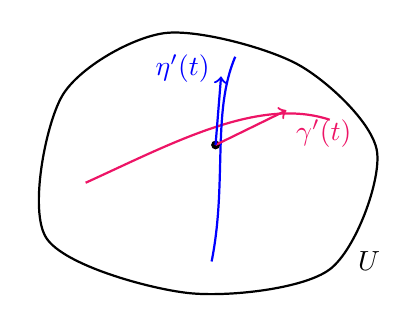
\begin{tikzpicture}[scale=1.0]
 \draw[thick] plot[smooth cycle] coordinates
  {(-2.2,-0.9) (-2.0,0.9) (-0.7,1.7) (1.0,1.3) (2.0,0.2) (1.4,-1.3) (-0.4,-1.6)};
 \draw[WildStrawberry,thick] (-1.7,-0.2) .. controls (-0.6,0.3) and (0.5,0.9) .. (1.4,0.6);
 \draw[blue,thick] (-0.1,-1.2) .. controls (0.1,-0.2) and (-0.1,0.7) .. (0.2,1.4);
 \fill (-0.05,0.28) circle (1.6pt);
 \draw[WildStrawberry,->,thick] (-0.05,0.28)--(0.85,0.72);
 \draw[blue,->,thick] (-0.05,0.28)--(0.02,1.15);
 \node[WildStrawberry,below right] at (0.85,0.72) {$\gamma'(t)$};
 \node[blue,left] at (0.0,1.25) {$\eta'(t)$};
 \node at (1.9,-1.2) {$U$};
\end{tikzpicture}
\end{center}

\begin{remark}
If $\gamma'(t)\ne0$, then $\bigl(-y'(t),x'(t)\bigr)$ is a normal vector to
$\gamma$ at $t$.
\end{remark}

Now let $f:U\to\C$ be holomorphic on $U$. Composing, we obtain a new curve
$f\circ\gamma$ in the image:
\be
 [a,b]\xrightarrow{\ \gamma\ }U\xrightarrow{\ f\ }\C,
 \qquad t\longmapsto f(\gamma(t)).
\ee

\begin{center}
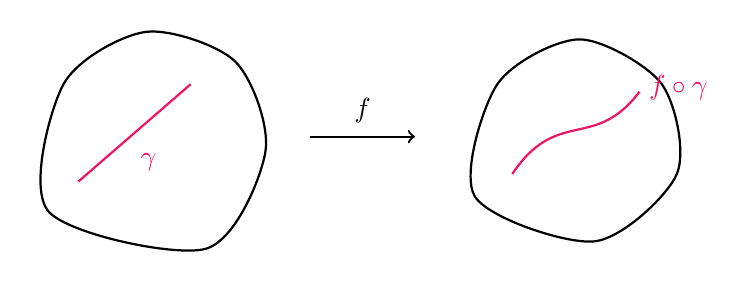
\begin{tikzpicture}[scale=0.95]
 \draw[thick] plot[smooth cycle] coordinates
  {(-2.3,-0.8) (-2.1,0.9) (-1.0,1.6) (0.2,1.2) (0.6,0.0) (-0.2,-1.3)};
 \draw[WildStrawberry,thick] (-1.9,-0.4)--(-0.4,0.9);
 \node[WildStrawberry,below right] at (-1.2,0.1) {$\gamma$};
 \draw[->,thick] (1.2,0.2)--(2.6,0.2);
 \node[above] at (1.9,0.25) {$f$};
 \begin{scope}[shift={(5.0,0)}]
  \draw[thick] plot[smooth cycle] coordinates
   {(-1.6,-0.6) (-1.3,0.9) (-0.2,1.5) (0.9,0.9) (1.1,-0.3) (0.0,-1.2)};
  \draw[WildStrawberry,thick] (-1.1,-0.3) .. controls (-0.5,0.6) and (0.0,0.0) .. (0.6,0.8);
  \node[WildStrawberry,right] at (0.6,0.85) {$f\circ\gamma$};
 \end{scope}
\end{tikzpicture}
\end{center}

\begin{example}[Chain rule]
\label{ex:chain-rule}
For a differentiable curve $\gamma$ and $f$ holomorphic,
\be
 \frac{d}{dt}f(\gamma(t))=f'(\gamma(t))\cdot\gamma'(t).
\ee
\emph{Proof:} Regard $f$ as the associated real map
$F=(u,v):U\to\R^2$ and apply the multivariable chain rule to $F\circ\gamma$.
The Cauchy--Riemann equations identify the real derivative of $F$ with
multiplication by $f'(\gamma(t))$.
\end{example}

% Handwritten page 5.
\subsection{Angles between curves}
Now suppose we are given two curves
\be
 \gamma:[a,b]\to U,\qquad \eta:[c,d]\to U,
\ee
and assume that at a point of intersection
\be
 z_0=\gamma(t_0)=\eta(s_0),
 \qquad \gamma'(t_0)\ne0,\quad \eta'(s_0)\ne0.
\ee

\begin{center}
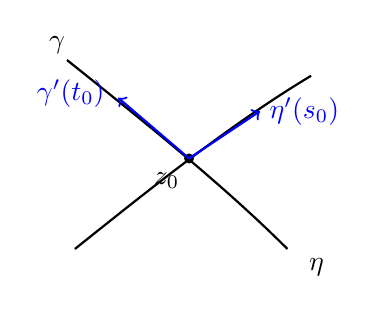
\begin{tikzpicture}[scale=1.0]
 \draw[thick] (-1.6,1.2) .. controls (-0.6,0.4) and (0.4,-0.4) .. (1.2,-1.2);
 \draw[thick] (-1.5,-1.2) .. controls (-0.5,-0.4) and (0.5,0.4) .. (1.5,1.0);
 \fill (-0.05,-0.05) circle (1.8pt);
 \node[below left] at (-0.05,-0.1) {$z_0$};
 \draw[blue,->,thick] (-0.05,-0.05)--(0.85,0.55);
 \node[blue,right] at (0.85,0.55) {$\eta'(s_0)$};
 \draw[blue,->,thick] (-0.05,-0.05)--(-0.95,0.72);
 \node[blue,left] at (-1.0,0.77) {$\gamma'(t_0)$};
 \node[above left] at (-1.5,1.15) {$\gamma$};
 \node[below right] at (1.35,-1.2) {$\eta$};
\end{tikzpicture}
\end{center}

\begin{definition}
The \emph{oriented angle from $\gamma$ to $\eta$ at $z_0$} is the oriented
angle from $\gamma'(t_0)$ to $\eta'(s_0)$, taken modulo $2\pi$.
\end{definition}

\begin{lemma}
\label{lem:conformal}
Assume $f'(z_0)\ne0$. Then the oriented angle from $f\circ\gamma$ to
$f\circ\eta$ at $f(z_0)$ is equal to the oriented angle from $\gamma$ to
$\eta$ at $z_0$.
\end{lemma}

\begin{remark}
A map which preserves angles in this way is called \emph{conformal}.
So the lemma says: holomorphic $\Longrightarrow$ conformal (at points where
the derivative does not vanish).
\end{remark}

% Handwritten page 6.
\begin{proof}
By Example~\ref{ex:chain-rule}, the tangent vectors of the image curves at
$t_0$ are
\be
 \frac{d}{dt}f(\gamma(t))\Big|_{t_0}=f'(z_0)\,\gamma'(t_0),
 \qquad
 \frac{d}{ds}f(\eta(s))\Big|_{s_0}=f'(z_0)\,\eta'(s_0),
\ee
where $\gamma(t_0)=\eta(s_0)=z_0$.

\begin{center}
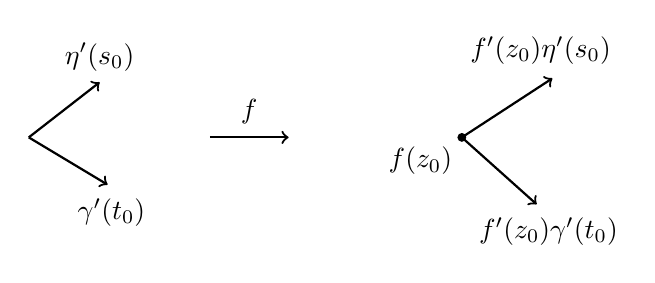
\begin{tikzpicture}[scale=1.0]
 \draw[->,thick] (-0.9,0.0)--(0.0,0.7);
 \node[above] at (0.0,0.72) {$\eta'(s_0)$};
 \draw[->,thick] (-0.9,0.0)--(0.1,-0.6);
 \node[below] at (0.15,-0.65) {$\gamma'(t_0)$};
 \draw[->,thick] (1.4,0.0)--(2.4,0.0);
 \node[above] at (1.9,0.05) {$f$};
 \begin{scope}[shift={(4.6,0)}]
  \fill (0,0) circle (1.6pt);
  \node[below left] at (0,0) {$f(z_0)$};
  \draw[->,thick] (0,0)--(1.15,0.75);
  \node[above] at (1.0,0.8) {$f'(z_0)\eta'(s_0)$};
  \draw[->,thick] (0,0)--(0.95,-0.85);
  \node[below] at (1.1,-0.9) {$f'(z_0)\gamma'(t_0)$};
 \end{scope}
\end{tikzpicture}
\end{center}

Now $f'(z_0)$ is a nonzero complex number. Writing
$f'(z_0)=\rho e^{i\theta}$ with $\rho>0$, multiplication by $f'(z_0)$ is a
rotation by $\theta$ followed by a scaling by $\rho$. Both operations
preserve the oriented angle from $\gamma'(t_0)$ to $\eta'(s_0)$.
\end{proof}

\section{Green's theorem and complex analysis}
\begin{theorem}[Green's theorem]
\label{thm:green}
Let $U$ be a bounded region in $\R^2$ whose positively oriented boundary
$\partial U$ is piecewise $C^1$, and let
$F=\bigl(P(x,y),Q(x,y)\bigr)$ be a vector field whose components have
continuous first partial derivatives on an open set containing $\overline U$.
Then
\be
 \int_{\partial U}P\,dx+Q\,dy
 =\iint_U\left(\frac{\partial Q}{\partial x}-\frac{\partial P}{\partial y}\right)dx\,dy.
\ee
The left-hand side is the circulation integral of $F$ along the boundary.
\end{theorem}

\begin{center}
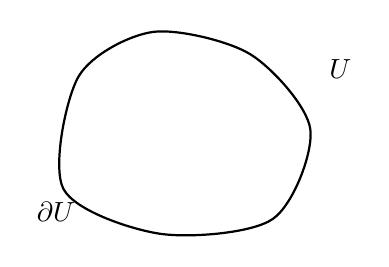
\begin{tikzpicture}[scale=0.95]
 \draw[thick] plot[smooth cycle] coordinates
  {(-1.8,-0.7) (-1.6,0.8) (-0.6,1.4) (0.7,1.1) (1.5,0.1) (1.0,-1.1) (-0.5,-1.3)};
 \node at (1.9,0.9) {$U$};
 \node at (-1.9,-1.0) {$\partial U$};
\end{tikzpicture}
\end{center}

% Handwritten page 7.
We first recall the definition of a complex line integral.

\begin{definition}
Let $\gamma:[a,b]\to U$ be a piecewise $C^1$ curve,
$\gamma(t)=x(t)+iy(t)$.
The \emph{line integral of $f$ along $\gamma$} is
\be
 \int_\gamma f(z)\,dz:=\int_a^b f(\gamma(t))\,\gamma'(t)\,dt.
\ee
\end{definition}

Expanding into real and imaginary parts, with
$f(\gamma(t))\gamma'(t)=(u+iv)(x'+iy')$, we obtain
\begin{align*}
 \int_\gamma f(z)\,dz
 &=\int_a^b\bigl(u(x(t),y(t))x'(t)-v(x(t),y(t))y'(t)\bigr)\,dt\\
 &\quad+i\int_a^b\bigl(u(x(t),y(t))y'(t)+v(x(t),y(t))x'(t)\bigr)\,dt.
\end{align*}

\begin{theorem}[Cauchy's theorem, first form]
\label{thm:cauchy-green}
Let $D\subseteq\C$ be a bounded region whose positively oriented boundary
$\partial D$ is piecewise $C^1$. Suppose $f=u+iv$ is defined on an open set
containing $\overline D$, is holomorphic there, and has continuous first
partial derivatives. Then
\be
 \boxed{\int_{\partial D}f(z)\,dz=0.}
\ee
\end{theorem}

\begin{proof}
Suppose
\be
 G=\bigl(\underbrace{u(x,y)}_{P},\ \underbrace{-v(x,y)}_{Q}\bigr).
\ee
Then by Green's theorem (Theorem~\ref{thm:green}),
\be
 \int_{\partial D}P\,dx+Q\,dy
 =\iint_D\bigl(-v_x-u_y\bigr)\,dx\,dy=0
\ee
by the Cauchy--Riemann equations, since $u_y=-v_x$.

On the other hand, by the expansion above,
\be
 \Real\left(\int_{\partial D}f(z)\,dz\right)
 =\int_{\partial D}P\,dx+Q\,dy=0.
\ee

Similarly, taking $P=v$ and $Q=u$, Green's theorem gives
\be
 \Imag\left(\int_{\partial D}f(z)\,dz\right)
 =\iint_D\bigl(u_x-v_y\bigr)\,dx\,dy=0,
\ee
again by the Cauchy--Riemann equations, since $u_x=v_y$.

Therefore
\be
 \int_{\partial D}f(z)\,dz=0.
\ee
\end{proof}

\begin{center}
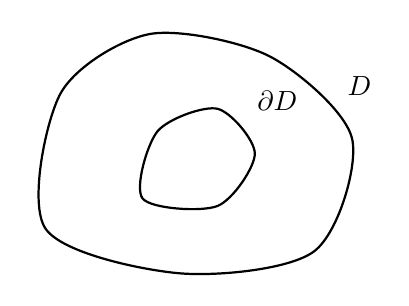
\begin{tikzpicture}[scale=0.95]
 \draw[thick] plot[smooth cycle] coordinates
  {(-2.2,-0.9) (-2.0,0.9) (-0.8,1.7) (0.8,1.4) (1.9,0.3) (1.4,-1.2) (-0.4,-1.5)};
 \draw[thick] plot[smooth cycle] coordinates
  {(-0.9,-0.5) (-0.7,0.4) (0.1,0.7) (0.6,0.1) (0.1,-0.6)};
 \node at (0.9,0.8) {$\partial D$};
 \node at (2.0,1.0) {$D$};
\end{tikzpicture}
\end{center}

\begin{remark}
This is a first version of \emph{Cauchy's theorem}: the integral of a
holomorphic function around a closed curve bounding a region inside the
domain vanishes. Note that the argument above needs the hypotheses of
Green's theorem, in particular continuity of the partial derivatives of $u$
and $v$. Removing this extra hypothesis requires a different proof, which we
will take up later.
\end{remark}

\end{document}
